\label{ch:collection}

%               ROADMAP
% =====================================
%
% we decided to use a commercial product
% movisens and the edamove4
%     - movisens ok
%     - edamove4 ok
%     - sensor usage and data retrieval ok
%     - unisens data format 
%     - accessory tools
% data Collection (falls performed and the hospital context)
% results
%

In order to further investigate the result obtained during the first experimentation session, a second testing trial was performed. This allowed the collection of additional data in order to draw conclusions in relation to the \textbf{feasibility} of the Electrodermal Activity analysis for classification purposes in the context of fall detection.

In this case, a commercial and publicly acknowledged device was employed in order to overcome the issues concerning the sensitivity to shocks and impacts of the BITalino device and, in addition, to acquire further bio-signals along with the Electrodermal Activity data.

\section{Movisens GmbH and the EdaMove Sensor}\label{sec:movisens}

The device employed consists of the \textbf{EdaMove4} sensor by \textbf{Movisens GmbH}, which is one of the most accurate and popular wearable devices aimed at the Electrodermal Activity measurement together with other such as the previously mentioned \textbf{Empatica E4}. Therefore, the following sections propose a brief overview of the product and its features.

\subsection{The company}\label{subsec:movisens-company}


Movisens GmbH is a German company deemed as a global leader in ambulatory assessment solutions \cite{movisens}, which offers several services such as workshops, consults, customized products and software in order to both support researchers and provide technologies and solutions for the healthcare sector.
The current catalog offers several sensor units for data collection and different mobile and desktop applications for data integration, processing and analysis. More specifically, the table \ref{toc:movisens-products} provides a list of the current available products.

\begin{table}[H]
\centering
\begin{tabular}{ll}
    \hline
    Name                     &  Description \\
    \hline
    \textbf{Move 4}          & A 10-Axis IMU that integrates a temperature sensor \\
    \textbf{EcgMove 4}       & A Move 4 unit that integrates ECG data collection  \\
    \textbf{EdaMove 4}       & A Move 4 unit that integrates EDA data collection \\
    \textbf{LightMove 4}     & A Move 4 unit that integrates the acquisition of ambient light measurements \\
    \textbf{SensorTrigger}   & A mobile solutions for activity-triggered data logging \\
    \textbf{movisensXS}      & A mobile solutions for Experience Sampling purposes \\
    \textbf{DataMerger}      & A desktop-based application for the integration of heterogeneous data \\
    \textbf{DataAnalyzer}    & A desktop-based application to analyze and report the acquired data \\
    \hline
\end{tabular}
\caption{List of products offered by Movisens GmbH}
\label{toc:movisens-products}
\end{table}

Moreover, the company provides several solutions that allow researchers and students to utilize the needed instrumentation by requiring a free, limited rent for a specific product. In this case, the company has consented a rental related to the \textbf{EdaMove 4} sensor for the required period of time. 

\subsection{The EdaMove 4 Sensor}\label{subsec:edamove4}

Across all the products developed by Movisens, the EdaMove 4 is the one that implements measurement functionalities for the Electrodermal Activity. It consists of a 62,3 x 38,6 x 11,5 mm case with a 26 g weight \cite{edamove4} that provides a Micro-USB connection (in order to connect the unit to the \textit{Sensor Manager} software) and two snap-button connectors in order to attach the positive and negative electrode. Moreover, a proper wrist band with pre-connected electrodes and specific mount points for the EdaMove 4 sensor allows the device to be worn seamlessly on the wrist or the ankle.


\begin{figure}[htp]
    \centering
    \subfloat[Electrodes Placement]{%
        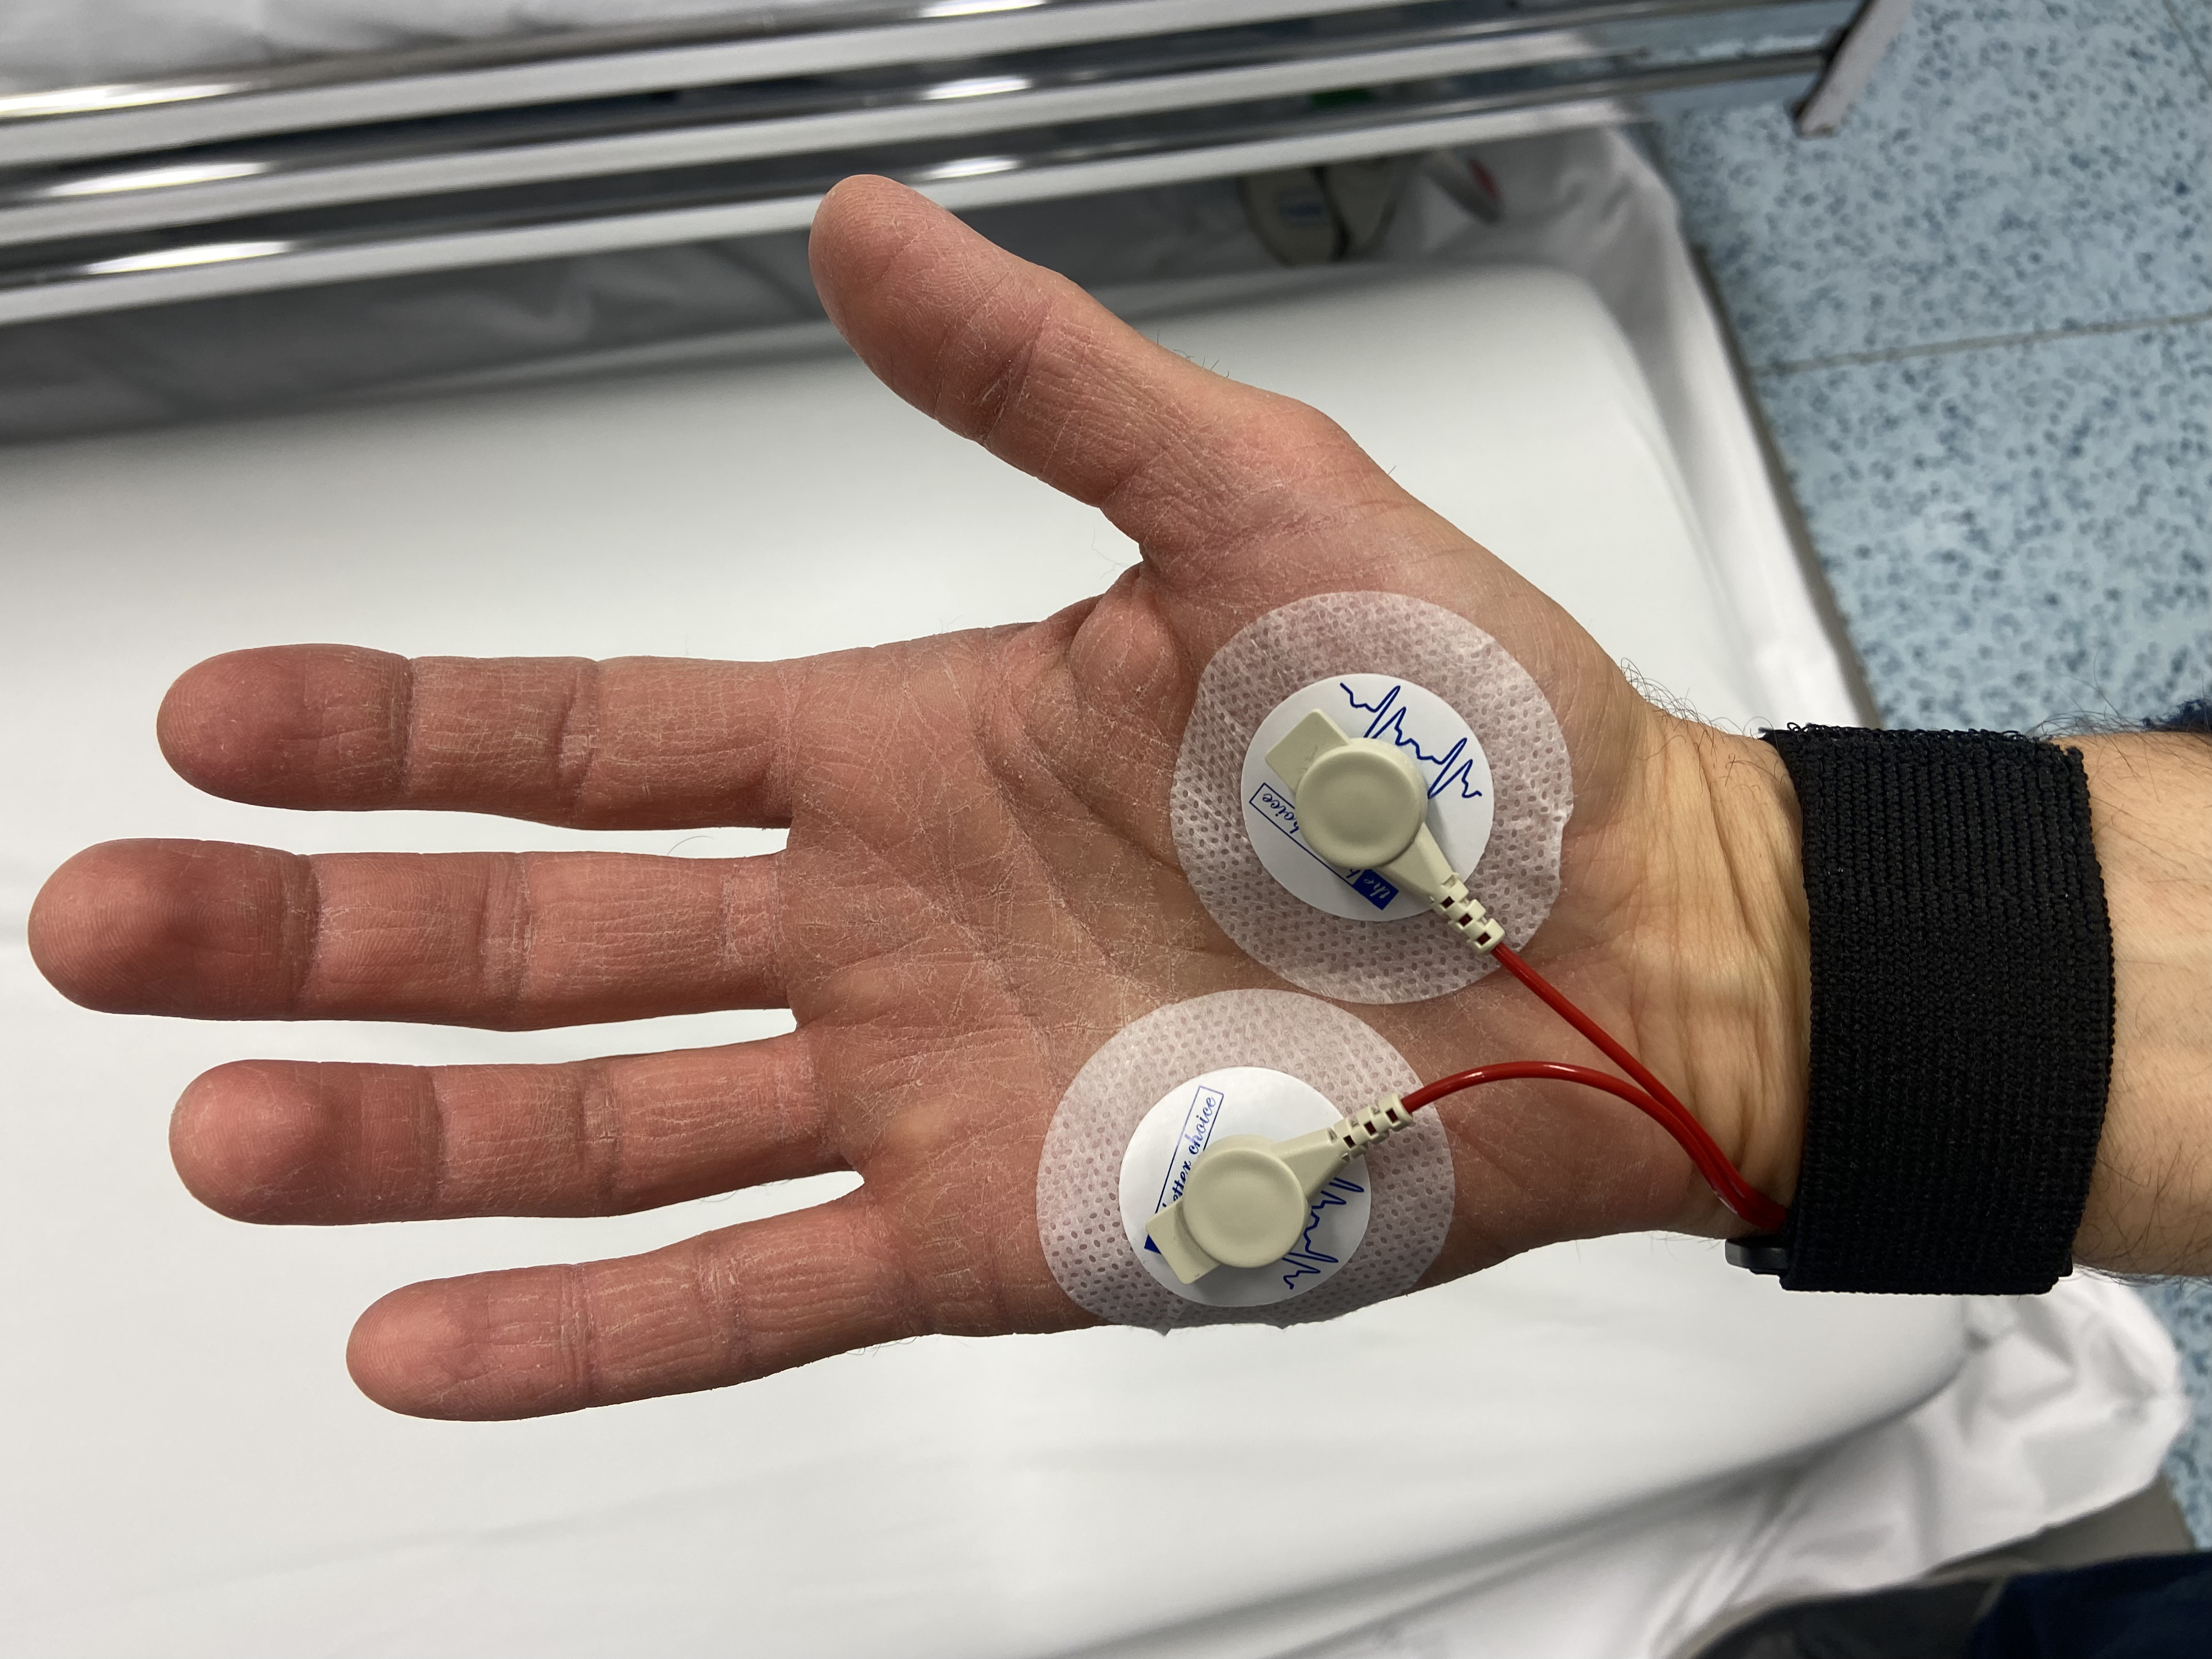
\includegraphics[width=0.4\textwidth]{./images/edamove1.jpeg}%
        \label{fig:edamovesensor-up}%
    }%
    \hfill%
    \subfloat[Electrodes Placement]{%
        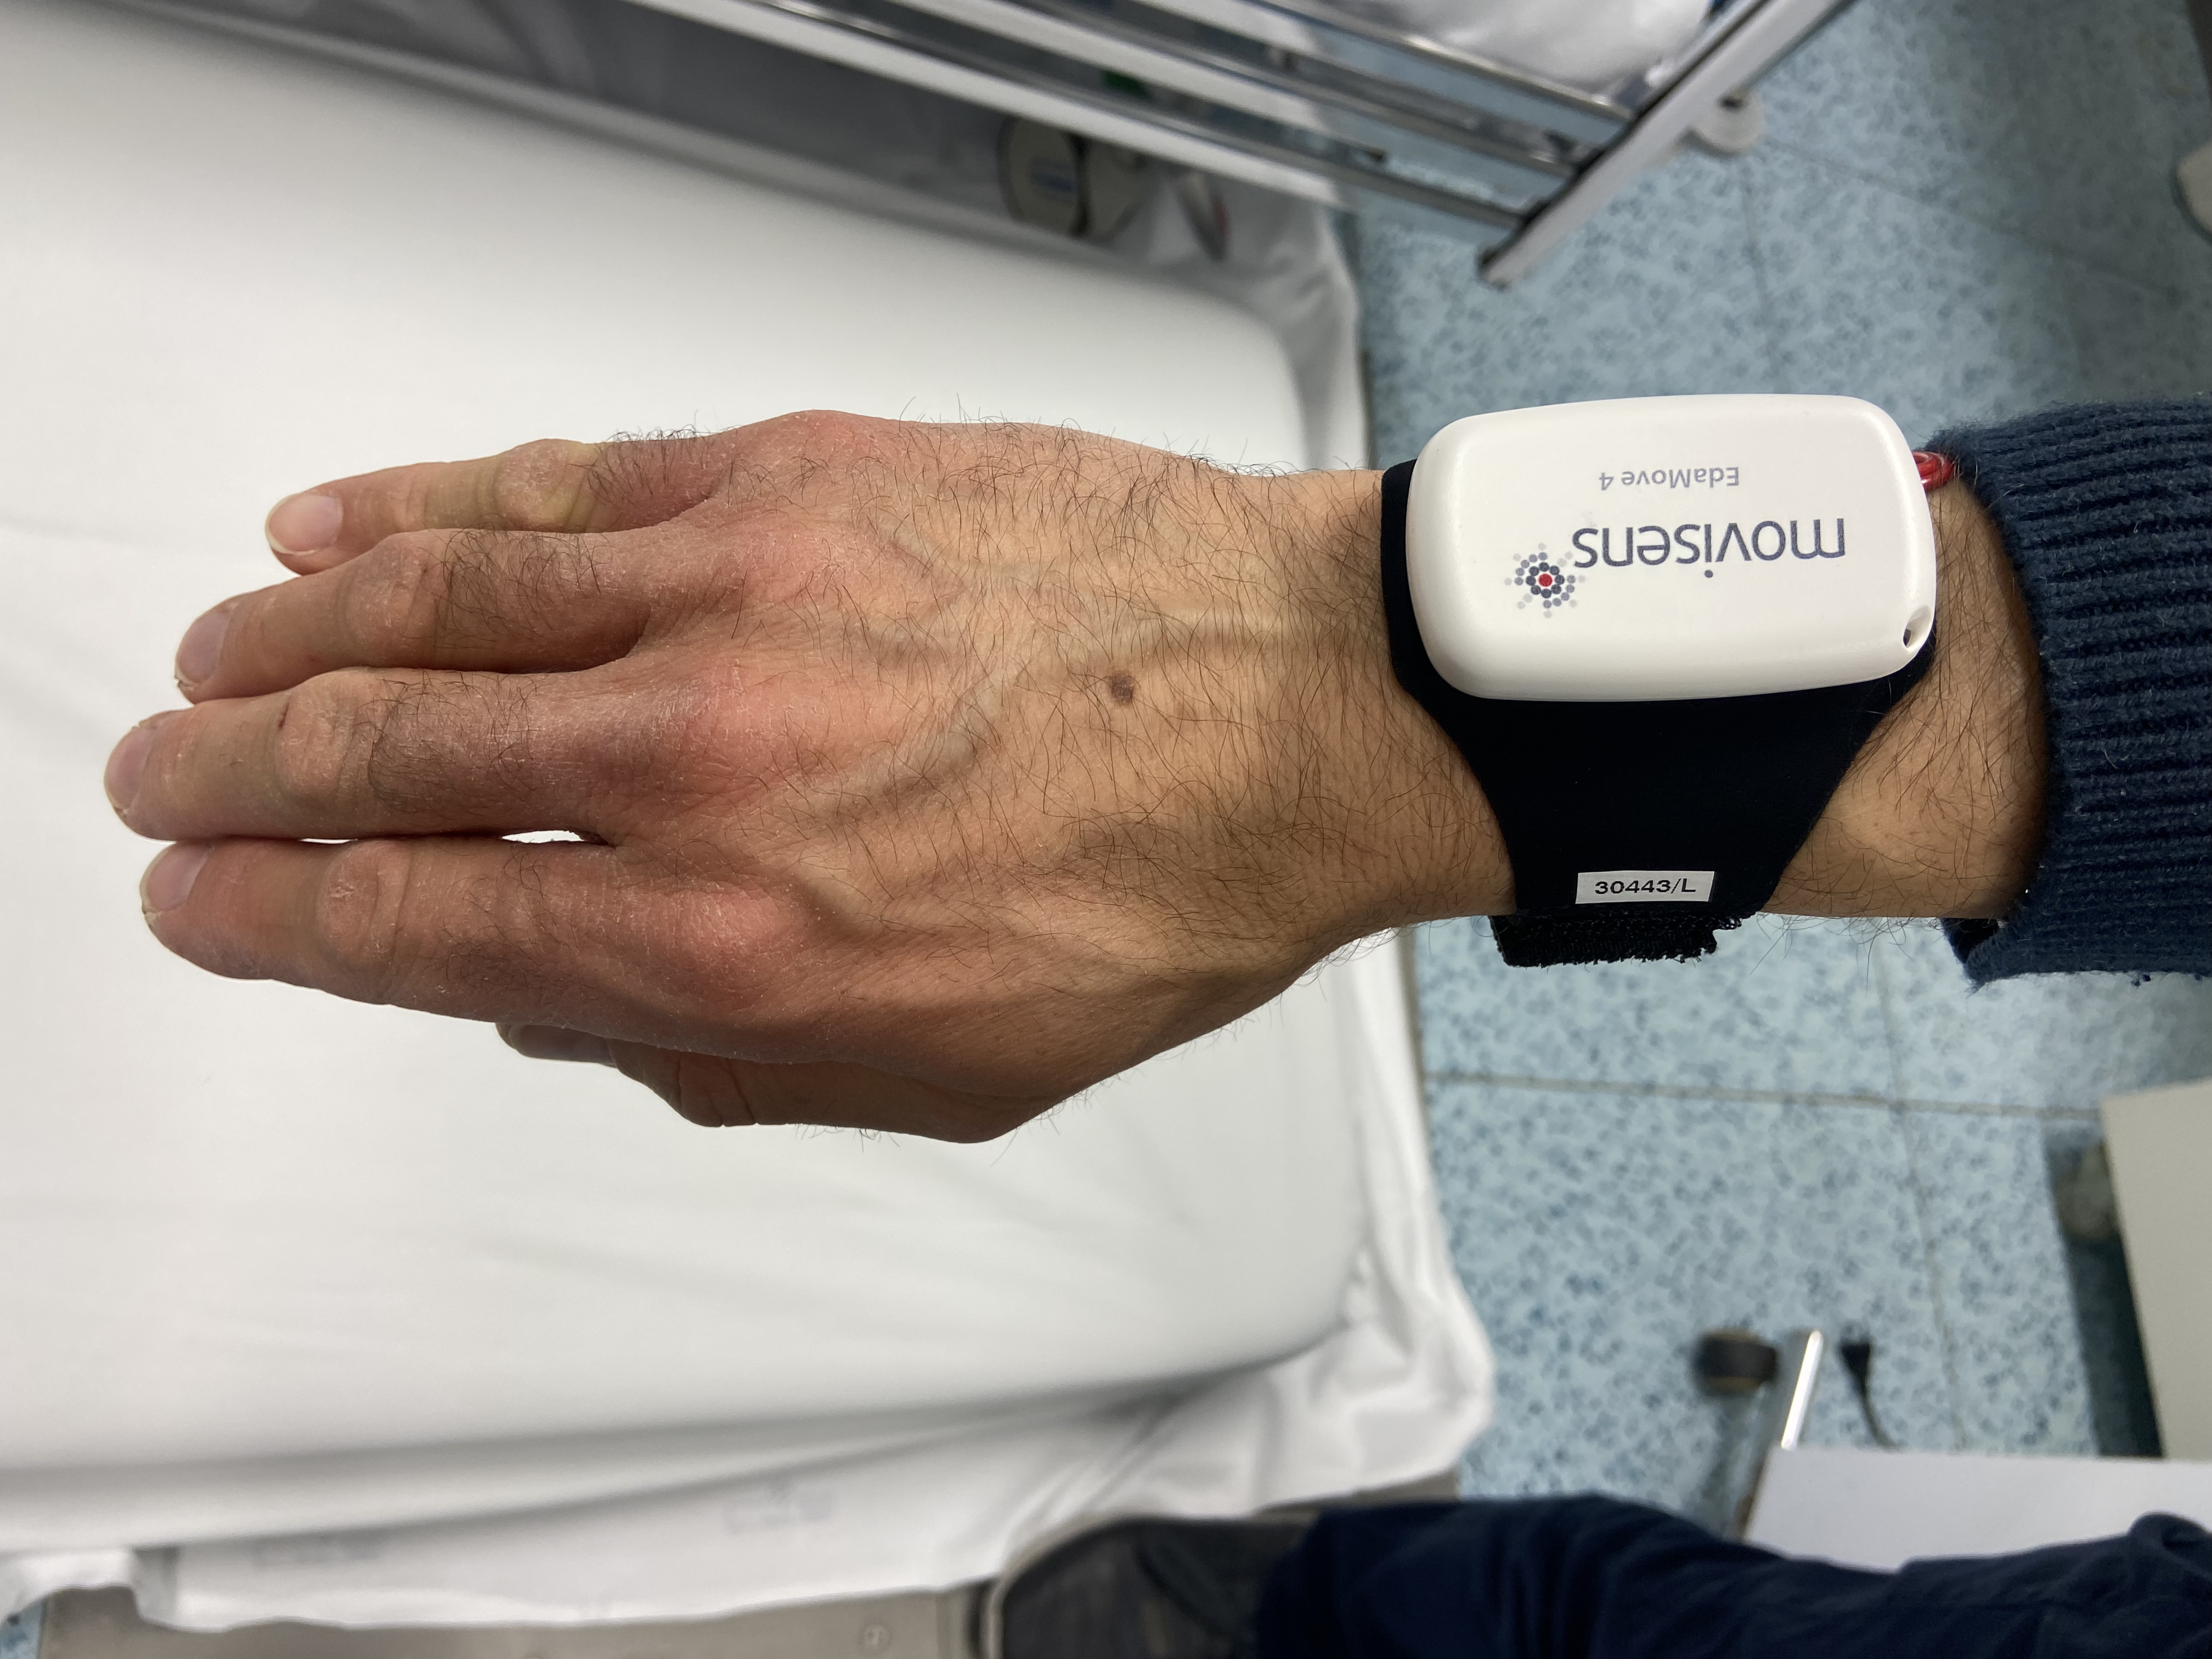
\includegraphics[width=0.4\textwidth]{./images/edamove2.jpeg}%
        \label{fig:edamovesensor-up}%
    }%
    \caption{The EdaMove 4 Sensor}
\end{figure}

Other than acquiring EDA measurement, the unit also offers:

\begin{itemize}
    \item A \textbf{3D Accelerometer}
    \item A \textbf{Rotation Rate} sensor
    \item A \textbf{Pressure} sensor
    \item A \textbf{Temperature} sensor
\end{itemize}

More specifically, the unit implements an exosomatic acquisition technique by applying a standard voltage of 0.5 V DC. The internal Analog to Digital Converter provides a 14 bit resolution and the output rate corresponds to 32 Hz for a 8 Hz bandwidth.

Moreover, the 3D accelerometers provides a $\pm$ 16 g range with an output rate of 64 Hz, while the rotation rate sensor offers a $\pm$ 2000 dps range, with a 64 Hz output rate and a 70 mdps resolution. The pressure sensor provides, instead, a measurement range between 300 and 1100 hPa, with a 8 Hz output rate and a 0.03 hPa resolution. Finally, the temperature sensor provides an output rate of 1 Hz.

The EdaMove 4 mounts a capacious Lithium battery which provides a constant 3.7 voltage and offers a continuous runtime of almost four days. An internal memory of 4 Gigabytes provides, instead, a maximum recording capacity of 4 weeks, allowing the usage of the sensor in varied contexts, from controlled experimentations to uncontrolled, domestic environments. 

Finally, the EdaMove 4 has been employed in several scientific publications that overall validated its functionalities.

\subsection{Usage}\label{subsec:edamove4-usage}

In order to organise a measurement session and subsequently extract the obtained data, Movisens provides a specific software toolchain intended to offer a cross-compatibility with all the \textbf{Move} sensors. 

The sensors can be configured through the \textbf{Sensor Manager} software, which allows to define the personal data of the participant wearing the sensor and set specific parameter such as the \textbf{duration} and the \textbf{start time} for the measurement. Furthermore, the software detects whether the unit has non-retrieved measurements in its storage and provides the functionalities to download the collected data on the machine. More specifically, the data storage configuration can be set in order to match one of the two modalities proposed: 

\begin{itemize}
    \item Plain CSV files
    \item \textbf{Unisens} File Format 
\end{itemize}

Besides the inclusion of a CSV modality, the company highly suggests the usage of the Unisens format in order to exploit the features that the standard implements and because it is the only format compatible with the \textbf{Unisens Viewer} and the \textbf{Data Analyzer} software products. The Unisens Viewew consists of a free and convenient tool that allows to plot and pre-process the raw data encoded in the Unisens format, providing functionalities to edit the measurements timeline by removing unwanted parts and by setting specific markers in order to later identify events of interest.

The pre-processed and examined dataset obtained can, then, be analysed by employing the Data Analyzer, a paid software that implements several algorithms and data processing techniques for the various data sources provided by the Movisens products.


\subsection{The Unisens Data Format}\label{subsec:unisens}




